\documentclass[landscape]{article}
\usepackage{amssymb}
\usepackage[landscape]{geometry}
\usepackage{multicol}
%\usepackage{helvet}
\usepackage{color}
%\usepackage[xdvi,dvips]{graphicx}
\usepackage{graphicx}
\usepackage{amsfonts, amstext, amsmath}
\usepackage{wrapfig}
\usepackage{float}
\usepackage[export]{adjustbox}
\usepackage{tcolorbox}
\usepackage{times}
\usepackage{anyfontsize}
\usepackage{tikz}
\usepackage{graphicx}
\usetikzlibrary{calc}

\newtcolorbox{mybox}{boxrule=6pt}

\def\argmax{\qopname\relax n{argmax}}
\def\s{\mathbf s}
\def\x{\mathbf x}
\def\u{\mathbf u}
\def\y{\mathbf y}
\def\d{\mathbf d}
\def\boldzero{\mathbf 0}
\def\pibold{\mbox{\boldmath $\pi$}}
\newcommand{\normal}[2]{\ensuremath{\mathcal{N}\left(#1,#2\right)}}
\newcommand{\given}{\mid}

\newenvironment{itemizeNoSymbol}{%
\renewcommand{\labelitemi}{}\begin{itemize}
\setlength{\itemsep}{1pt}
\setlength{\parskip}{0pt}
\setlength{\parsep}{0pt}}{\end{itemize}}


% set horizontal margins to center text (using current paperwidth &
% textwidth)
\newcommand{\equalmargins} {
\setlength{\oddsidemargin}{\paperwidth}
\addtolength{\oddsidemargin}{-\textwidth}
\setlength{\oddsidemargin}{0.5 \oddsidemargin}
\addtolength{\oddsidemargin}{-1in}
}

\setlength{\evensidemargin}{\oddsidemargin}

\renewcommand{\familydefault}{\sfdefault}

\input posterfonts.tex

% setup large (poster-sized) sheet
\setlength{\paperwidth}{200cm}
\setlength{\paperheight}{110cm}
%\pdfpagewidth\paperwidth
%\pdfpageheight\paperheight
 
\setlength{\textwidth}{195cm}
\setlength{\textheight}{105cm}
\setlength{\topmargin}{-.25truein}
 
\equalmargins
\setlength{\headsep}{0pt}
\setlength{\headheight}{0pt}

\pagestyle{empty}
\setlength{\parindent}{0mm}
\setlength{\parskip}{16pt}

% header style: title followed by a column-wide rule
\newcommand{\mysection}[1]{{\color[rgb]{.6,0,0}{\section*{{\HUGE #1}
        {\leaders\hrule height .2ex\hfill\kern0pt}}}}}

\begin{document}
\color{black}

% invisible rule is useful for spacing
\hrule width 0pt depth 0pt height 1pt

\begin{center}
  \titleSize
Degenerate solution networks for theoretical neuroscience \\
  \HUGE %
  Sean R. Bittner$^{1}$, Agostina Palmigiano$^1$, Kenneth D. Miller$^1$, John P. Cunningham$^2$ \\
  \huge
  $^{1}$Department of Neuroscience, Columbia University Medical Center,  $^{2}$ Department of Statistics, Columbia University
\end{center}

\begin{tikzpicture}[remember picture,overlay]
  \node[anchor=north east,inner sep=0pt, scale=0.5] at ($(current page.north east)+(-3cm,0cm)$) {
     
\includegraphics{figs/CU_logo}
  };
\end{tikzpicture}

\vspace{.5in}

\setlength{\columnsep}{1in}
\begin{multicols*}{4}

%%%%%%%%%%%%%%%%%%%%%%%%%%%%%%

\mysection{Motivation}
\LARGE
\begin{itemize}
\item Circuit models are often designed in the hopes of producing an emergent property observed in data (e.g., an oscillation, limit cycle, etc.)
\item However, the standard inference toolkit conditions on data, not this emergent property.
\item We develop degenerate solution networks (DSNs), a deep generative modeling approach to finding distributions over model parameters that produce a desired emergent behavior.
\item DSNs produce new insights into existing models and will become increasingly important as models get more complex.
\begin{multicols*}{2}
\item \textbf{Motivating example}: \\
What parameters of a 2D linear system...
\[\dot{x} = Ax \text{\hspace{.6in}} A = \begin{bmatrix} a_1 & a_2 \\ a_3 & a_4 \end{bmatrix} \text{\hspace{.6in}} z = \begin{bmatrix} a_1 \\ a_2 \\ a_3 \\ a_4 \end{bmatrix} \]
... yield a band of oscillations (the emergent property):
\begin{center}
\[E_{q(z)} \left[\omega_1 \right] = 1.0 Hz \]
\[Var_{q(z)}(\omega_1) = .025 Hz^2 \]
\end{center}


\columnbreak
\begin{center}
What we hope to find: \\
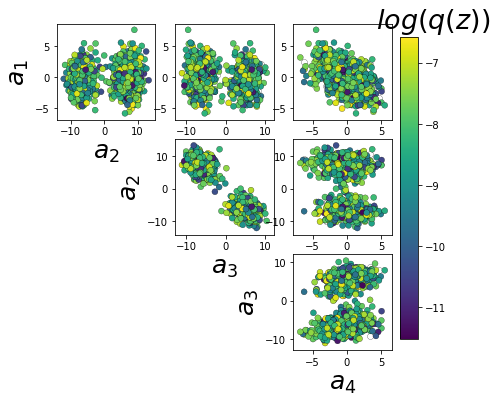
\includegraphics[scale=1.2]{figs/linear_2D.png}
\end{center}
\end{multicols*}

\end{itemize}
\vspace{-1in}

\mysection{Methods}
{\huge \textbf{Background: Deep generative modeling}}
\begin{multicols*}{2}
\vspace{-1in}
\begin{itemize}
\item By optimizing deep networks to map (approximately) a simple random distribution to a target distribution, we learn a distribution from a deep generative model. \\
\item \textbf{Max-entropy flow networks:} We can optimize DGMs to approximate max-ent distributions that satisfy sets of constraints (Loaiza-Ganem et al. 2018).
\end{itemize}
{\Large
 \begin{equation*}
\argmax_{q_\theta \in Q} H(q_\theta) \text{\hspace{.4in} s.t. } E_{q_\theta} \left[T(z) \right] = \mu 
\end{equation*}}

\columnbreak

{\LARGE
\begin{center}
\adjincludegraphics[clip, trim={0 0 0 0},scale=1.6]{figs/DGM.pdf}
\end{center}}
\end{multicols*}

\columnbreak

\begin{mybox}
{\huge \textbf{Degenerate solution networks}}
\begin{itemize}
\item DSNs are deep generative models of max-ent distributions of  parameterizations $z \sim q_\theta(z)$ yielding behavior $E_{z \sim q_\theta(z)} \left[ E_{p(x \mid z)} \left[T(x) \right] \right] = \mu$, for choice of model $p(x \mid z)$ and behavior $T(x)$.
\end{itemize}
\vspace{1cm}
\begin{center}
\adjincludegraphics[clip, trim={0 0 0 0},scale=1.4]{figs/DSN_red.pdf}
\end{center}

\begin{itemize}
\item DSNs enable: exploratory analyses, scientific hypothesis testing, and experimental design.
\end{itemize}
\end{mybox}

\mysection{Application 1: 4-neuron V1 model}
\hspace{10in} (Dipoppa et al. 2018)
\vspace{-.5in}
\begin{center}
\adjincludegraphics[clip, trim={0 0 0 0},scale=0.9]{figs/V1_model.pdf}
\hspace{1in}
\adjincludegraphics[clip, trim={0 0 0 0},scale=0.9]{figs/dipoppa.pdf}
\end{center}

\begin{multicols*}{2}
\begin{center}
{\LARGE \textbf{Emergent properties:}} \\
{\large \textbf{Modulation with locomotion:}} \\
\adjincludegraphics[clip, trim={0 0 0 0},scale=0.7]{figs/V1_behavior_summary.pdf}
\end{center}
\columnbreak
\textbf{Model:}
\[r = \begin{bmatrix} r_E \\ r_P \\ r_S \\ r_V \end{bmatrix} \text{\hspace{.5in}} \tau \frac{dr}{dt} = -r + [Wr + h]_+^n\]
\vspace{.05in}
\begin{itemize}
\item What parameterizations of this model yield these emergent properties?
\end{itemize}

\end{multicols*}

\columnbreak

{\bf\huge DSN for small stimuli circuit behavior} \\
\vspace{-.75in}
\begin{center}
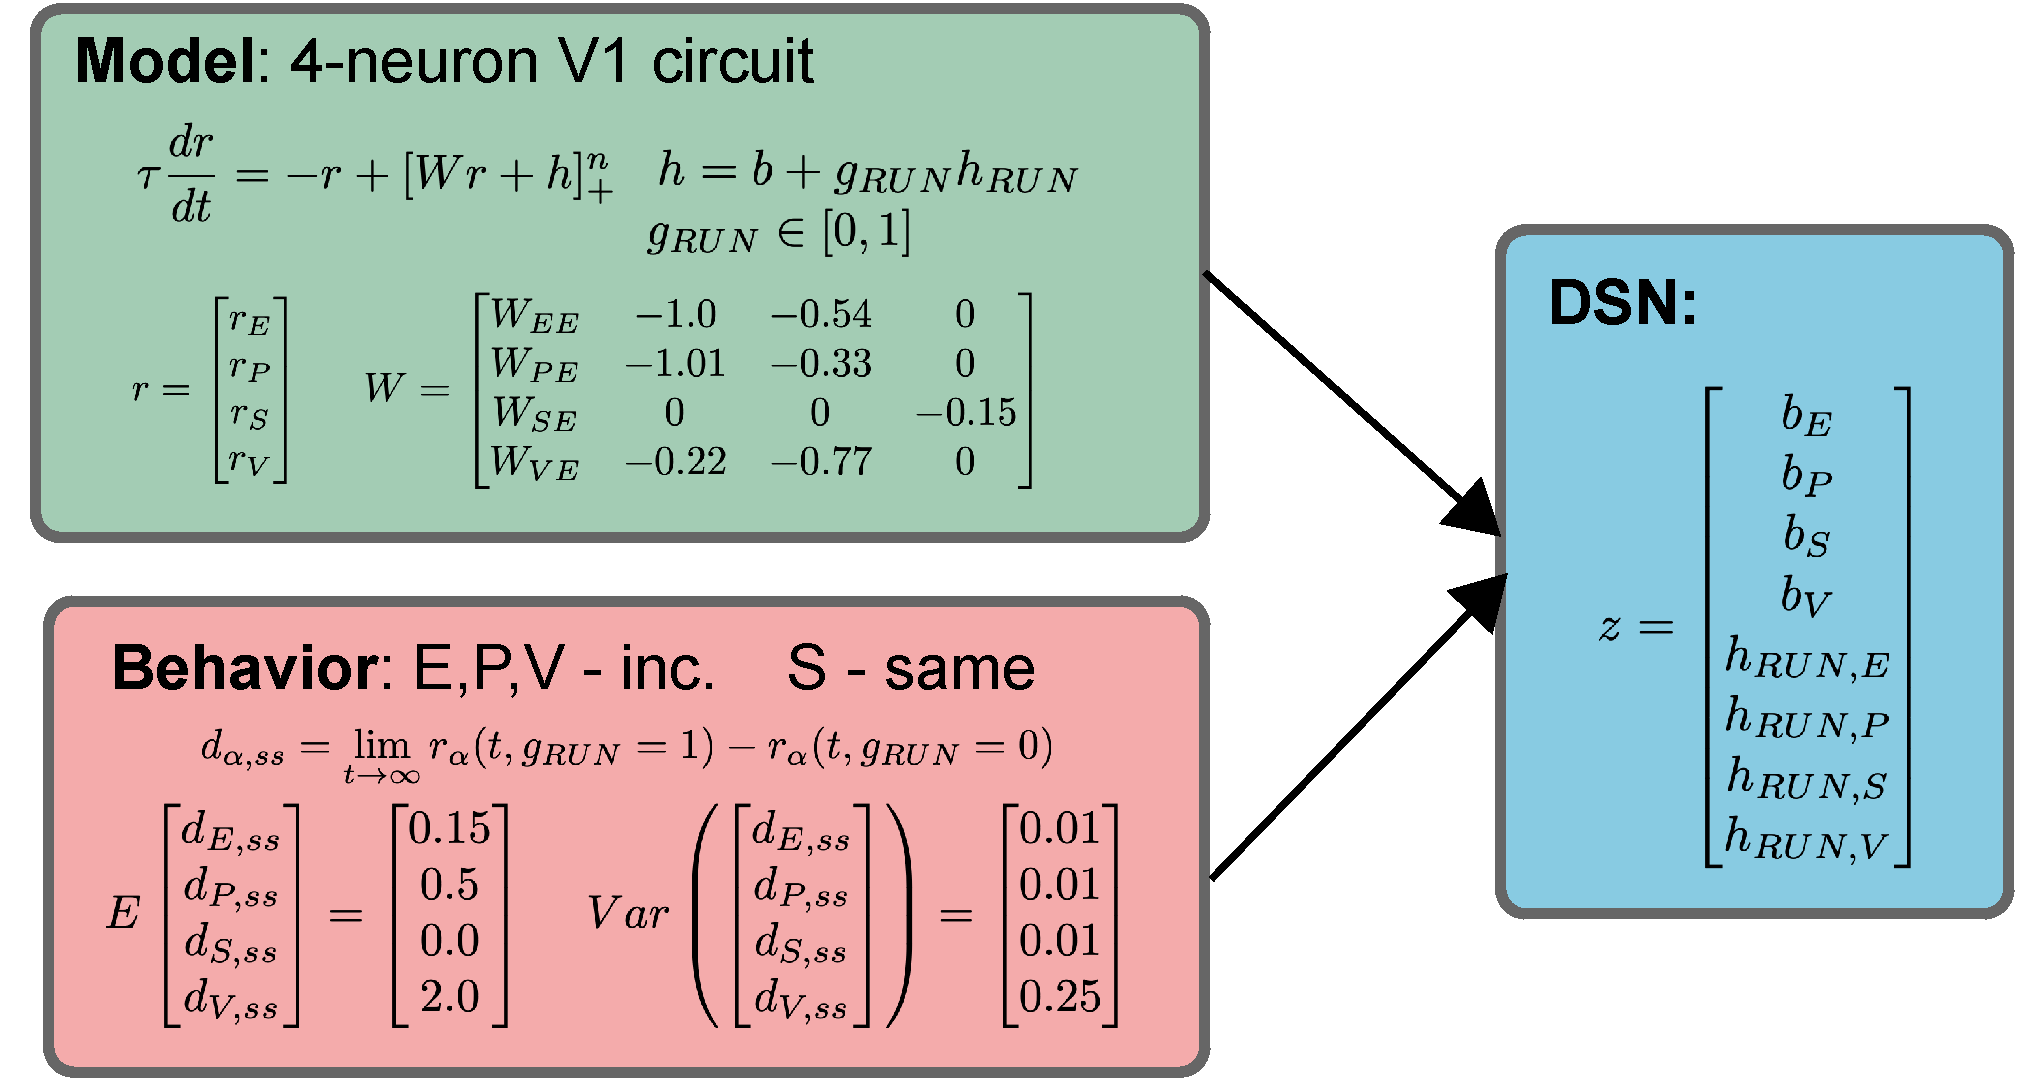
\includegraphics[scale=1.0]{figs/V1_DSN.pdf} \\
\end{center}

\begin{multicols*}{2}
{\bf\huge Samples:} \\
\vspace{-1.75in}
\begin{center}
\adjincludegraphics[clip, trim={0 0 0 0},scale=0.85]{figs/V1_DSN_samples.pdf}
\end{center}

\columnbreak
\begin{mybox}
{\bf\huge Novel insight from DSN:} \\
\begin{itemize}
\item $b_E$ increases $d_{P,ss}$.
\begin{center}
\adjincludegraphics[clip, trim={0 0 0 0},scale=0.85]{figs/corr4.png}
\end{center}
\item $b_P$, $b_S$, $b_V$ suppresses $d_{E,ss}$.
\begin{center}
\adjincludegraphics[clip, trim={0 0 0 0},scale=0.5]{figs/I_corrs.pdf}
\end{center}
\end{itemize}
\end{mybox}
\end{multicols*}

\mysection{Application 2: Low rank RNNs}
\begin{itemize}
\item We can design low rank RNNs to solve common neuroscientific tasks by casting mean field variables into task-relevant ones \\ (Mastrogiuseppe et al. 2018).
\end{itemize}
\begin{multicols*}{2}
{\bf\LARGE Model:} 
\[\dot{x}_i(t) = -x_i(t) + \sum_{j=1}^N J_{ij} \phi(x_j(t)) + I_i\]
\[J_{ij} = g \chi_{ij} + P_{ij} \]
\[\chi_{ij} \sim \mathcal{N}(0, \frac{1}{N}) \text{\hspace{1in}} P_{ij} = \sum_{k=1}^r \frac{m_i^{(k)}n_j^{(k)}}{N} \]

\columnbreak

{\bf\LARGE Dynamic mean field theory:} 
\[ \dot{x}_i(t) = -x_i(t) + \eta_i(t)\]
\[\mu = \langle \left[x_i \right] \rangle \text{\hspace{.5in}} \Delta_0 = \langle \left[x_i^2 \right] \rangle - \langle \left[x_i \right] \rangle^2 \]
\[\kappa_i = \frac{1}{N}\sum_{j=1}^N n_j^{(i)} \left[\phi_j \right] \text{\hspace{.5in}} \Delta_T = \Delta_0 - \Delta_\infty \]


\end{multicols*}

{\bf\huge Structured chaotic networks:} 
\vspace{-.5in}
\begin{center}
\adjincludegraphics[clip, trim={0 0 0 0},scale=0.8]{figs/StructChaos_DSN.pdf}
\end{center}

\columnbreak

{\bf\huge Noisy Detection:}  \\
\adjincludegraphics[clip, trim={0 0 0 0},scale=0.9]{figs/ND_DSN.pdf}

{\bf\huge Context dependent discrimination:}  \\
\adjincludegraphics[clip, trim={0 0 0 0},scale=0.9]{figs/CDD_DSN.pdf}

\begin{mybox}
{\bf\huge Novel insight from DSN:} 
\begin{multicols*}{2}
In rank-1 noisy detection networks $\Sigma_m$ suppresses chaos.
\begin{center}
\adjincludegraphics[clip, trim={0 0 0 0},scale=1.2]{figs/ND_insight.png}
\end{center}

\columnbreak


In rank-2 context-dep. RNNs $\gamma_{HI}$ increases chaos $\Delta_T$.
\begin{center}
\adjincludegraphics[clip, trim={0 0 0 0},scale=1.2]{figs/CDD_insight.png}
\end{center}
\end{multicols*}
\end{mybox}

\mysection{Summary}
\begin{itemize}
\item Degenerate solution networks learn maximally expansive (max-entropy) dists of model parameters that yield emergent properties.
\item We show novel insight provided by DSNs for a 4-neuron nonlinear dynamical model of V1, and low-rank RNNs solving tasks.
\end{itemize}


\large

{\bf\Large References}

1. Loaiza-Ganem, G., Y. Gao., and J. P. Cunningham. ``Maximum entropy flow networks." ICLR (2017). \\
2. Dipoppa, M., et al. ``Vision and locomotion shape the interactions between neuron types in mouse visual cortex." Neuron (2018). \\
3. Mastrogiuseppe, F., and S. Ostojic. ``Linking connectivity, dynamics, and computations in low-rank recurrent neural networks." Neuron (2018).

{\bf\Large Acknowledgements} \\
NSF Graduate Research Fellowship,  DGE-1644869, McKnight Endowment Fund, NIH NINDS 5R01NS100066, Simons Foundation 542963, NSF 1707398, The Gatsby Charitable Foundation \\
Stephen Baccus, James Fitzgerald, and Dhruva Raman for helpful conversations.

\end{multicols*}
\end{document}
